%\title{DIY Scuba Diving Log Book}
% Author: Tom (texblog.org)
% Details: http://texblog.org/2015/07/22/diy-scuba-diving-log-book/
\documentclass[17pt,a4paper]{extarticle}
\usepackage[margin=0.7in]{geometry}
\usepackage{tikz, fancyhdr}
\usepackage{amssymb}\usepackage{rotating}
\linespread{2}
\pagestyle{fancy}
\fancyhf{}
\renewcommand{\headrulewidth}{0pt}
\rfoot{\scriptsize Created by texblog.org}
\makeatletter
\def\hrulefill{\leavevmode\leaders\hrule height 0.8pt\hfill\kern\z@}
\makeatother
\begin{document}
%%%%%%%%%%%%%
%General info and stamp
%%%%%%%%%%%%%

oindent
\begin{minipage}{0.6\linewidth}

oindent
Dive Nr \hrulefill\ Date \hrulefill\hrulefill\\
Location \hrulefill\\
Dive site \hrulefill
\end{minipage}
\qquad
\begin{minipage}{0.37\linewidth}
\fbox{\parbox[c][5cm][c]{5cm}{\hspace{5cm}}}\\
{\scriptsize Stamp}
\end{minipage}

\vspace{1cm}
%%%%%%%%%%%%%%%
%Profile and detail information
%%%%%%%%%%%%%%%

oindent
\begin{minipage}{0.55\linewidth}
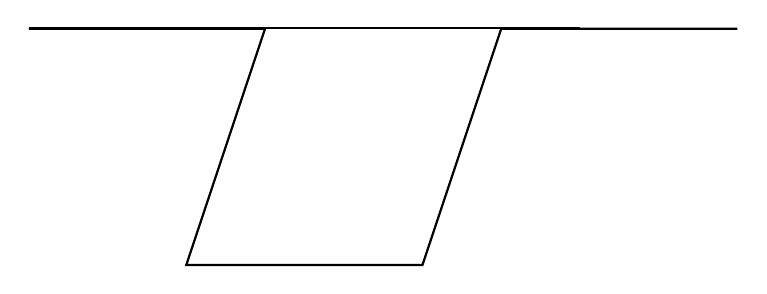
\begin{tikzpicture}
\draw[thick] (0,0) -- (3,0) -- (2,-3) -- (5,-3) -- (6,0) -- (9,0);

ode [text width=3cm, align=center] (time) at (1,-1.5) {\baselineskip=24pt Max\\depth\\\rule{2cm}{0.8pt}\par};

ode [align=center] (depth) at (4,-4) {Bottom time \rule{3cm}{0.8pt}\ min};

ode [text width=3cm, align=center] (stop) at (7.5,-1.5) {\baselineskip=24pt Safety\\stop\\\rule{2cm}{0.8pt}\par};
\end{tikzpicture}
\end{minipage}
\quad
\begin{minipage}{0.4\linewidth}

oindent
Weights \hrulefill\ kg/lb\\
$\square$ Long $\square$ Shorty \hrulefill\ mm\\
Temperature \hrulefill\\
Visibility \hrulefill\\
\end{minipage}

\vspace{1cm}

oindent
Comments \hrulefill\\
\phantom{}\hrulefill\\
\phantom{}\hrulefill\\
\phantom{}\hrulefill\\
\phantom{}\hrulefill\\
\phantom{}\hrulefill\\
$\square$ Instructor Nr \hrulefill\ $\square$ Dive master $\square$ Buddy\\
Name \hrulefill\ Sign \hrulefill
\end{document}